\section{Introduction}

Autonomous vehicles are considered to be one of the most challenging
types of reactive systems currently under development. They need to
interact with a highly reactive environment. Life critical decisions
have to be made instantaneously and need to be executed at the right
point in time. However, even if the intricate task of designing such
systems is conquered, that the result must be guaranteed to be also safe and reliable.

Program verification is not only applied in reactive settings, but also useful for verifying other mission-critical applications.
One major advancement from the programming languages community towards bug-free software has been the development of functional languages.
Functional languages use features to control the space of possible programs via abstraction, which can prevent many common programming errors.
For example, functional purity reduces the possibility of malformed state that can cause unexpected behavior.
In the simplest case, the higher-order function \texttt{map} common to functional languages is an abstraction for looping (among other functions) that eliminates the typical intermediate counter.
This helps to eliminate the possibility for runtime index out of bounds errors due to mistaken reasoning about edge cases.



explain that functional languages now also are used for hardware
  (embedded systems people probably don't know about that) (mention
  results like \emph{clash} or \emph{Kansas Lava})


for reactive systems, a proper notion of time is necessary,
  motivate on some example (synchronous vs asynchronous, real vs
  discrete), finally lead to FRP




In summary, we make the following contributions:

\begin{itemize}
\item An overview of Functional Reactive Programming (FRP) and how it allows for easier reasoning about correctness properties in reactive systems. 
\cfelix{this is the most important part, almost sure that nobody of the reviews will know about; go through the very basics, remember these are embedded systems people}

\item A library for connecting Haskell to the vehicle simulator TORCS, encouraging further research into the use of functional languages for the development of safer autonomous vehicle controllers.

\item A demonstration of an FRP controller for a vehicle that highlights the elegance and simplicity of the framework,
   which makes it resistant against errors. Furthermore it is easily extendable without breaking the remaining system.

\end{itemize}

\begin{figure}[t]
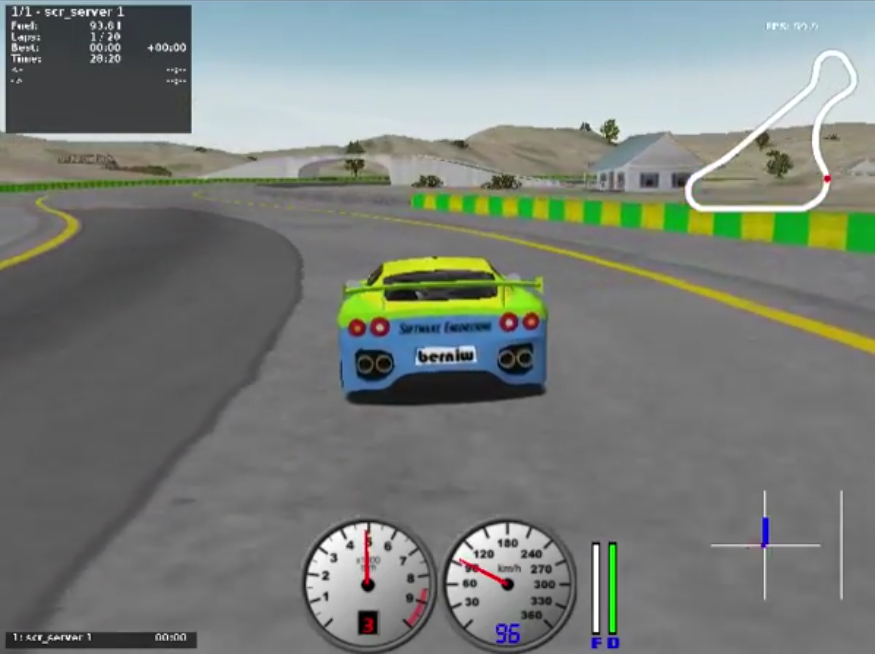
\includegraphics[width=0.45\textwidth]{figs/racing.png}
\caption{A screenshot of Haskell controlling the autonomous vehicle in the TORCS simulator}
\label{fig:race}
\end{figure}
